\section{Transversal intersections and the $\lambda-$lemma}
We found out that the (un-)stable sets are submanifolds of our compact Riemannian manifold that we started with. From a topological point of view we would love our \mbox{(un-)stable} sets to be closed as that would make them compact. From figure \ref{fig: The closure of (un-)stable sets} we can already deduce some assumptions on how the closures will look like and the goal of this chapter is to prove those. 
\begin{figure}[p!]
\centering
    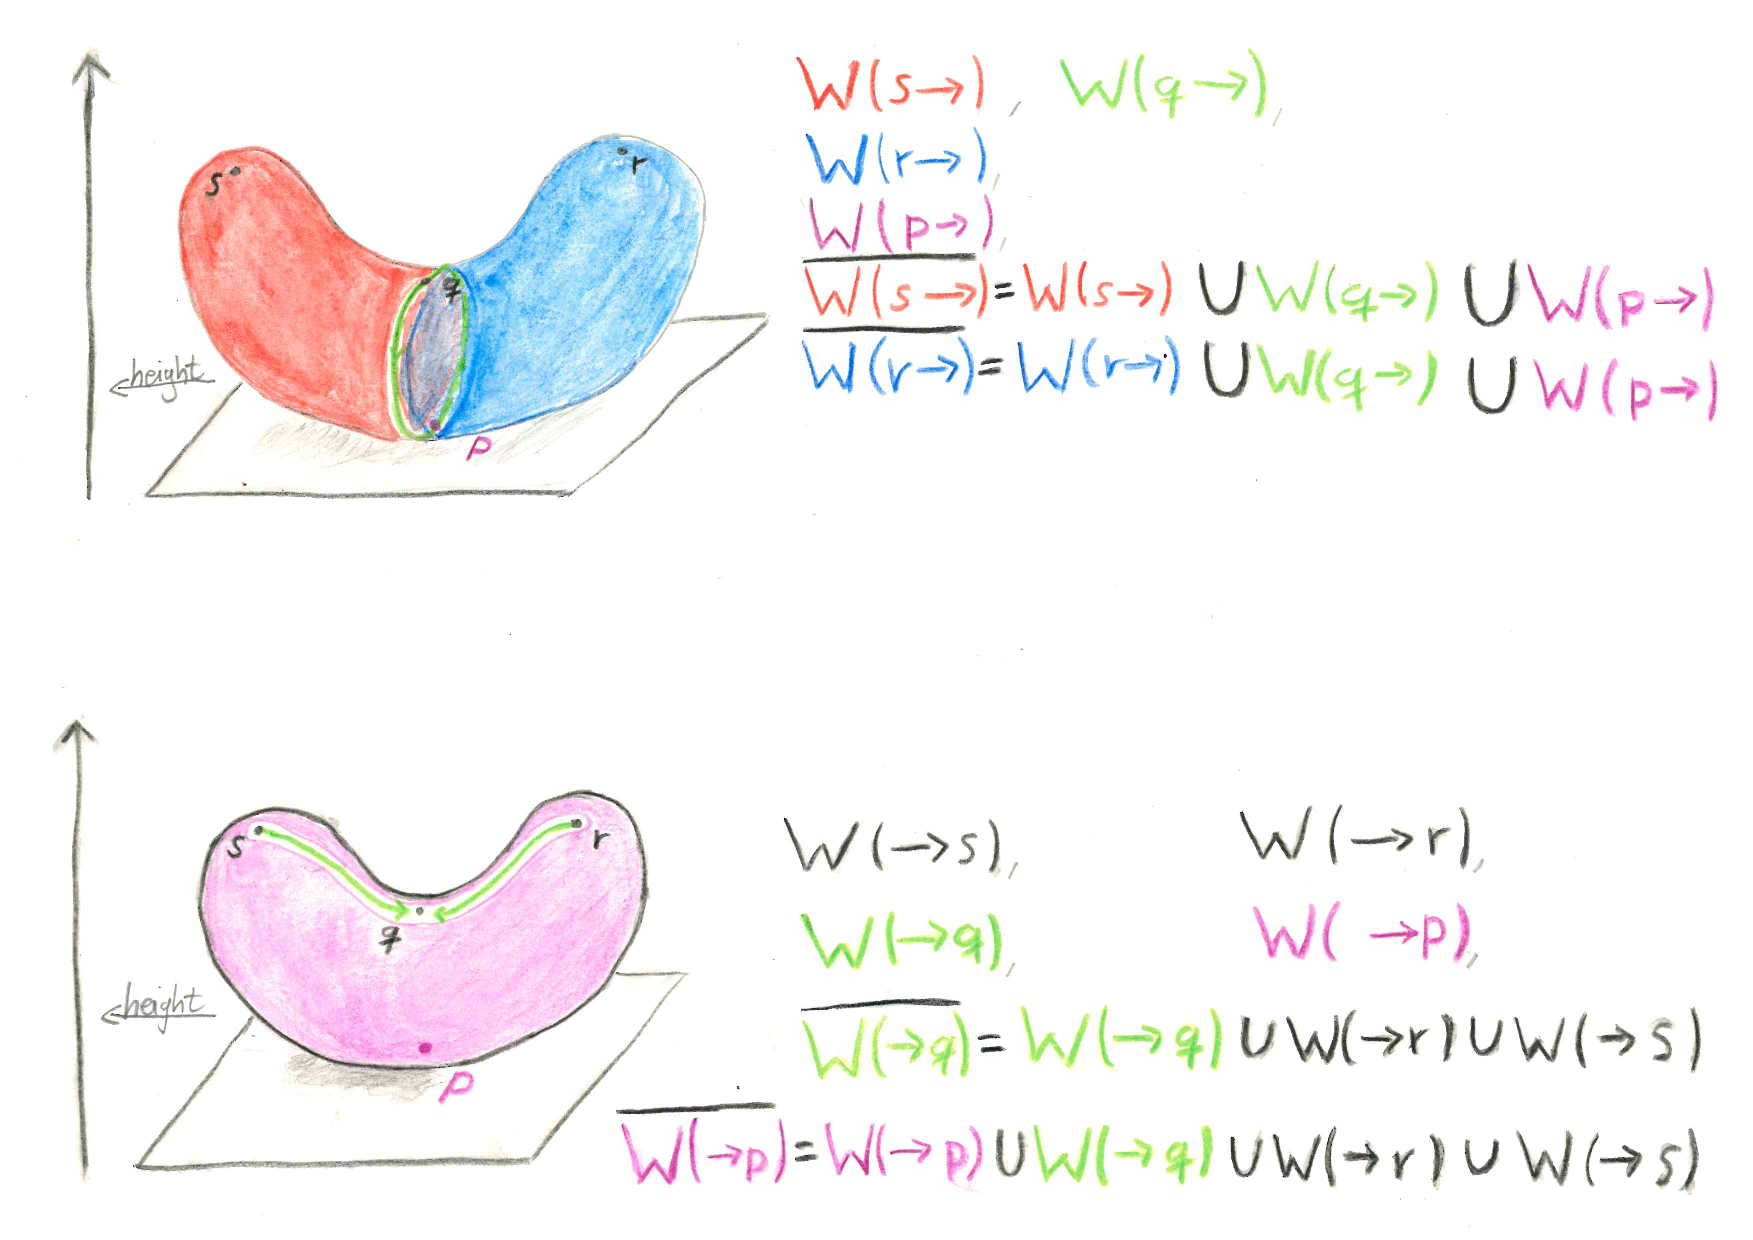
\includegraphics[width=0.9\textwidth]{Text/Pictures/lambdalemma/LambdaLemmaAnwendungen.pdf}
    \caption{The closure of (un-)stable sets.}
    \label{fig: The closure of (un-)stable sets}
\end{figure} \clearpage

\begin{definition}[Transversal intersection]
    Let $M,N,Z$ be smooth manifolds and $f:N \to M$, and $g:Z\to M$. 
    \begin{center}
        % https://tikzcd.yichuanshen.de/#N4Igdg9gJgpgziAXAbVABwnAlgFyxMJZARgBoAGAXVJADcBDAGwFcYkQBZEAX1PU1z5CKchWp0mrdgDkefEBmx4CRAExiaDFm0QgAWnP5KhRUcXFapugCqzeRwSpRlzmyTpDWu9hQOXDkdVcJbXZrA25xGCgAc3giUAAzACcIAFskMhAcCCRREKsQRMMi1IzEdWzcxHzLDxiQGkZ6ACMYRgAFPxNdZKwYgAscEpT0pABmGhzMn1HygFYp6tVZsqQAFiW81bHERaqNt1DdAB0TqCxExIACBqbW9q7jJxA+weGd8smDxE2CjzOFyu12KkW4QA
\begin{tikzcd}
N \arrow[r, "f"]                  & M            & Z \arrow[l, "g"']                  \\
TN \arrow[u] \arrow[r, "\diff f"] & TM \arrow[u] & TZ \arrow[u] \arrow[l, "\diff g"']
\end{tikzcd}
    \end{center}
    Then we say \textbf{$f$ intersects $g$ transversally } ($f \transcap g$) if for all $x,y,z:~f(x)=g(z)=y$ :
    \begin{equation*}
        \diff f|_x(T_xN)+\diff g|_z(T_zZ)=T_yM.
    \end{equation*} The sum here denotes the Minkowski sum. Two submanifolds intersect transversally if their inclusions intersect transversally.
\end{definition}




 \begin{definition}[Morse-Smale function]
     A Morse function $f:M\to \R$ is a \textbf{Morse-Smale} function, if for all critical points $p,q\in \Crit(f)$ the (un-)stable sets intersect transversally:
     \begin{equation*}
         W(\to p)\transcap W(q\to).
     \end{equation*}
 \end{definition}


 
 \begin{remark}[From $p$ to $q$] \label{rem: dimension from q to p }
 Let $f:M\to \R$ be a Morse-Smale function and $p,q\in \Crit(f)$. If $\underbrace{W(q\to)\cap W(\to p)}_{:=W(q\to p)} \neq \emptyset$ then $W(q\to p)$ is a submanifold of dimension $\ind_f(q)-\ind_f(p)$ or zero, if the difference is negative.
 \end{remark}
\begin{proof}
    First we note that by the (un-)stable manifold theorem \ref{thm: local (un-)stable manifold theorem} we have:
    \begin{align*}
        \dim(W(q\to))&=\ind_f(q), \\
        \dim(W(\to p))&=\dim(M)-\ind_f(p).
    \end{align*} Since $W(q\to)$ is a submanifold we can choose a chart $\phi: M\to \R^{\ind_f(q)}\times \R^{m-ind_f(q)}$, where $m=\dim(M)$, such that $\phi|_{W(q\to)}\subseteq \R^{\ind_f(q)}\times \{0\}$. Locally we obtain the projection 
    \begin{align*}
        \pi: M &\to V \subseteq \R^{m-\ind_f(q)}\\
        (x_1,...,x_{\ind_f(q)},y_{\ind_f(q)+1},...,y_m) &\mapsto (y_{\ind_f(q)+1},...,y_m),
    \end{align*}such that $\pi^{-1}(0)=W(\to q)$. Furthermore, we have the inclusion $i:W(\to p) \hookrightarrow M$. With this we define $$g:\pi \circ i:W(\to p) \to  V \subseteq \R^{m-\ind_f(q)}. $$ For $x\in M$ with $g(x)=0$ we know that $\diff g |_x$ is a surjection and $g^{-1}(\{0\})$ is a submanifold where $\text{codim} g^{-1}(\{0\})\subseteq W(\to p))=m-\ind_f(q)$. Therefore: \begin{align*}
       & \dim(W(\to p))-\dim(g^{-1}(\{0\})=m-\ind_f(q) \\ \Leftrightarrow \quad & m-\ind_f(p)-\dim(g^{-1}(\{0\})=m-\ind_f(q)\\
        \Leftrightarrow \quad &\dim(g^{-1}(\{0\})=\ind_f(q)-\ind_f(p).
    \end{align*}
    Obviously, $g^{-1}(\{0\})=W(q\to p)$ which concludes the proof.
\end{proof}






\begin{cor} \label{cor: lambda lemma flow lines have decreasing index}
    This tells us that two critical points $p,q$ of the same index either have a zero dimensional manifold connecting them or else none at all. Since a zero dimensional manifold would only contain discrete points a connection between two different critical points of the same index cannot exist. Furthermore those manifolds are path connected via the integral curves. Furthermore, if $W(q\to p)$ is not empty, it must contain a flow line of dimension one. But then $\ind_f(q)>\ind_f(p)$.
\end{cor}


\begin{remark}
The property of transverse intersection is kept under small perturbations of one of the manifolds. This \textit{metaproperty} is captured in the definition of stable properties:
\end{remark}
\begin{definition}[Stability of properties]
Given a property of a class of smooth maps ${f:M \to N}$ between two manifolds. Assume that for every $x\in M$ there is a neighbourhood $U$ of $x$ such that whenever  $f|_U$ possess that property and $H:U\times [0,1] \to N$ is a smooth homotopy of $f|_U$ then there exists an $\epsilon>0$ such that for all $t<\epsilon$ $H(\cdot,t)$ also possesses that property. In that situation we call that property \textbf{locally stable}.  If the property holds for $U=M$ we call the property \textbf{globally stable}.\end{definition}

\begin{theorem}[Stability Theorem]
If $M$ and $N$ are smooth manifolds then the following classes of smooth maps are locally stable:
\begin{enumerate}
\item Immersions,
\item submersions,
\item local diffeomorphisms,
\item maps transverse to a specified closed submanifold $Z\subseteq N$. 
\end{enumerate}
Furthermore, if $M$ is compact, then those classes are globally stable. 
\end{theorem}
\begin{proof}
Assume that $f:M\to N$ is an immersion and by choosing local coordinates we assume that $f:U \to V$ where $U\subset \R^m$ and $V\subset \R^n$ where both are open and $x\in U$. Let $H$ be a smooth homotopy of $f|_U$ and let $f_t(x):= H(x,t)$. The proof is just a matter of using continuity: Since $f_0$ is an immersion we know that its Jacobian has a $m\times m$-minor with non-zero determinant. Looking at this minor we notice that $f_t(x)$ is smooth in $x$ and $t$ and that the determinant is smooth. Therefore, a small neighbourhood of $0\in [0,1]$ exists where this determinant does not vanish. Thus the property \textit{immersion} is locally stable. For submersions consider a $n \times n$ minor and for diffeomorphisms note that they are immersions where the dimensions agree. Finally for the transverse intersection we consider the restriction  ${f:f^{-1}(U \times V)\to (U\times V)}$, where ${U\times \{0\} \subset Z}$. The property of transverse intersection reads that ${\diff f_x(T_xM)+T_{f(x)}V=T_xN}$. The last is equivalent to ${g=\pi_V\circ f:f^{-1}(U \times V)\to V }$ restricted to $g^{-1}(0)$ being a submersion. Now let $H$ be a smooth homotopy of $f$ and $f_t(x)=H(x,t)$. Then $\tilde{H}:= \pi_V\circ H$ is a smooth homotopy with $\tilde{H}(x,0)=g(x)$. Since being a submersion is a local stable property we can find an $\epsilon$ such that $\tilde{H(x,t)}$ is a submersion for all $t<\epsilon$. Then for all those $t$ we conclude that the restrictions of $\tilde{H}(\cdot ,t)$ to $\tilde{H}(\cdot,t)^{-1}(0)$ are submersions letting us conclude that $H(\cdot,t)$  intersects $U\times \{0\}$ transversely. Global stability follows from compactness by taking a finite sub cover that covers $M$ and the minimal $\epsilon$. 
\end{proof}







Next we want to get a notion of \textit{close by} for functions. Therefore, we look at the following definition of a topology, that considers functions to be close, if their first $r$ derivatives are point-wise close.
\begin{definition}[$C^r-$Topology]
Let $C^r(M,N)$ denote the space of $C^r-$maps between two $C^r-$manifolds. Let $(\phi,U)$ and $(\psi,V)$ be charts of $M,N$ into $\R^m$ respectively $\R^n$. Let $K\subseteq M$ be a compact set in $U$ such that $f(K)\subseteq V$. This setup is shown in figure \ref{fig: The C^r topology}.

\begin{figure}[p!]
\centering
    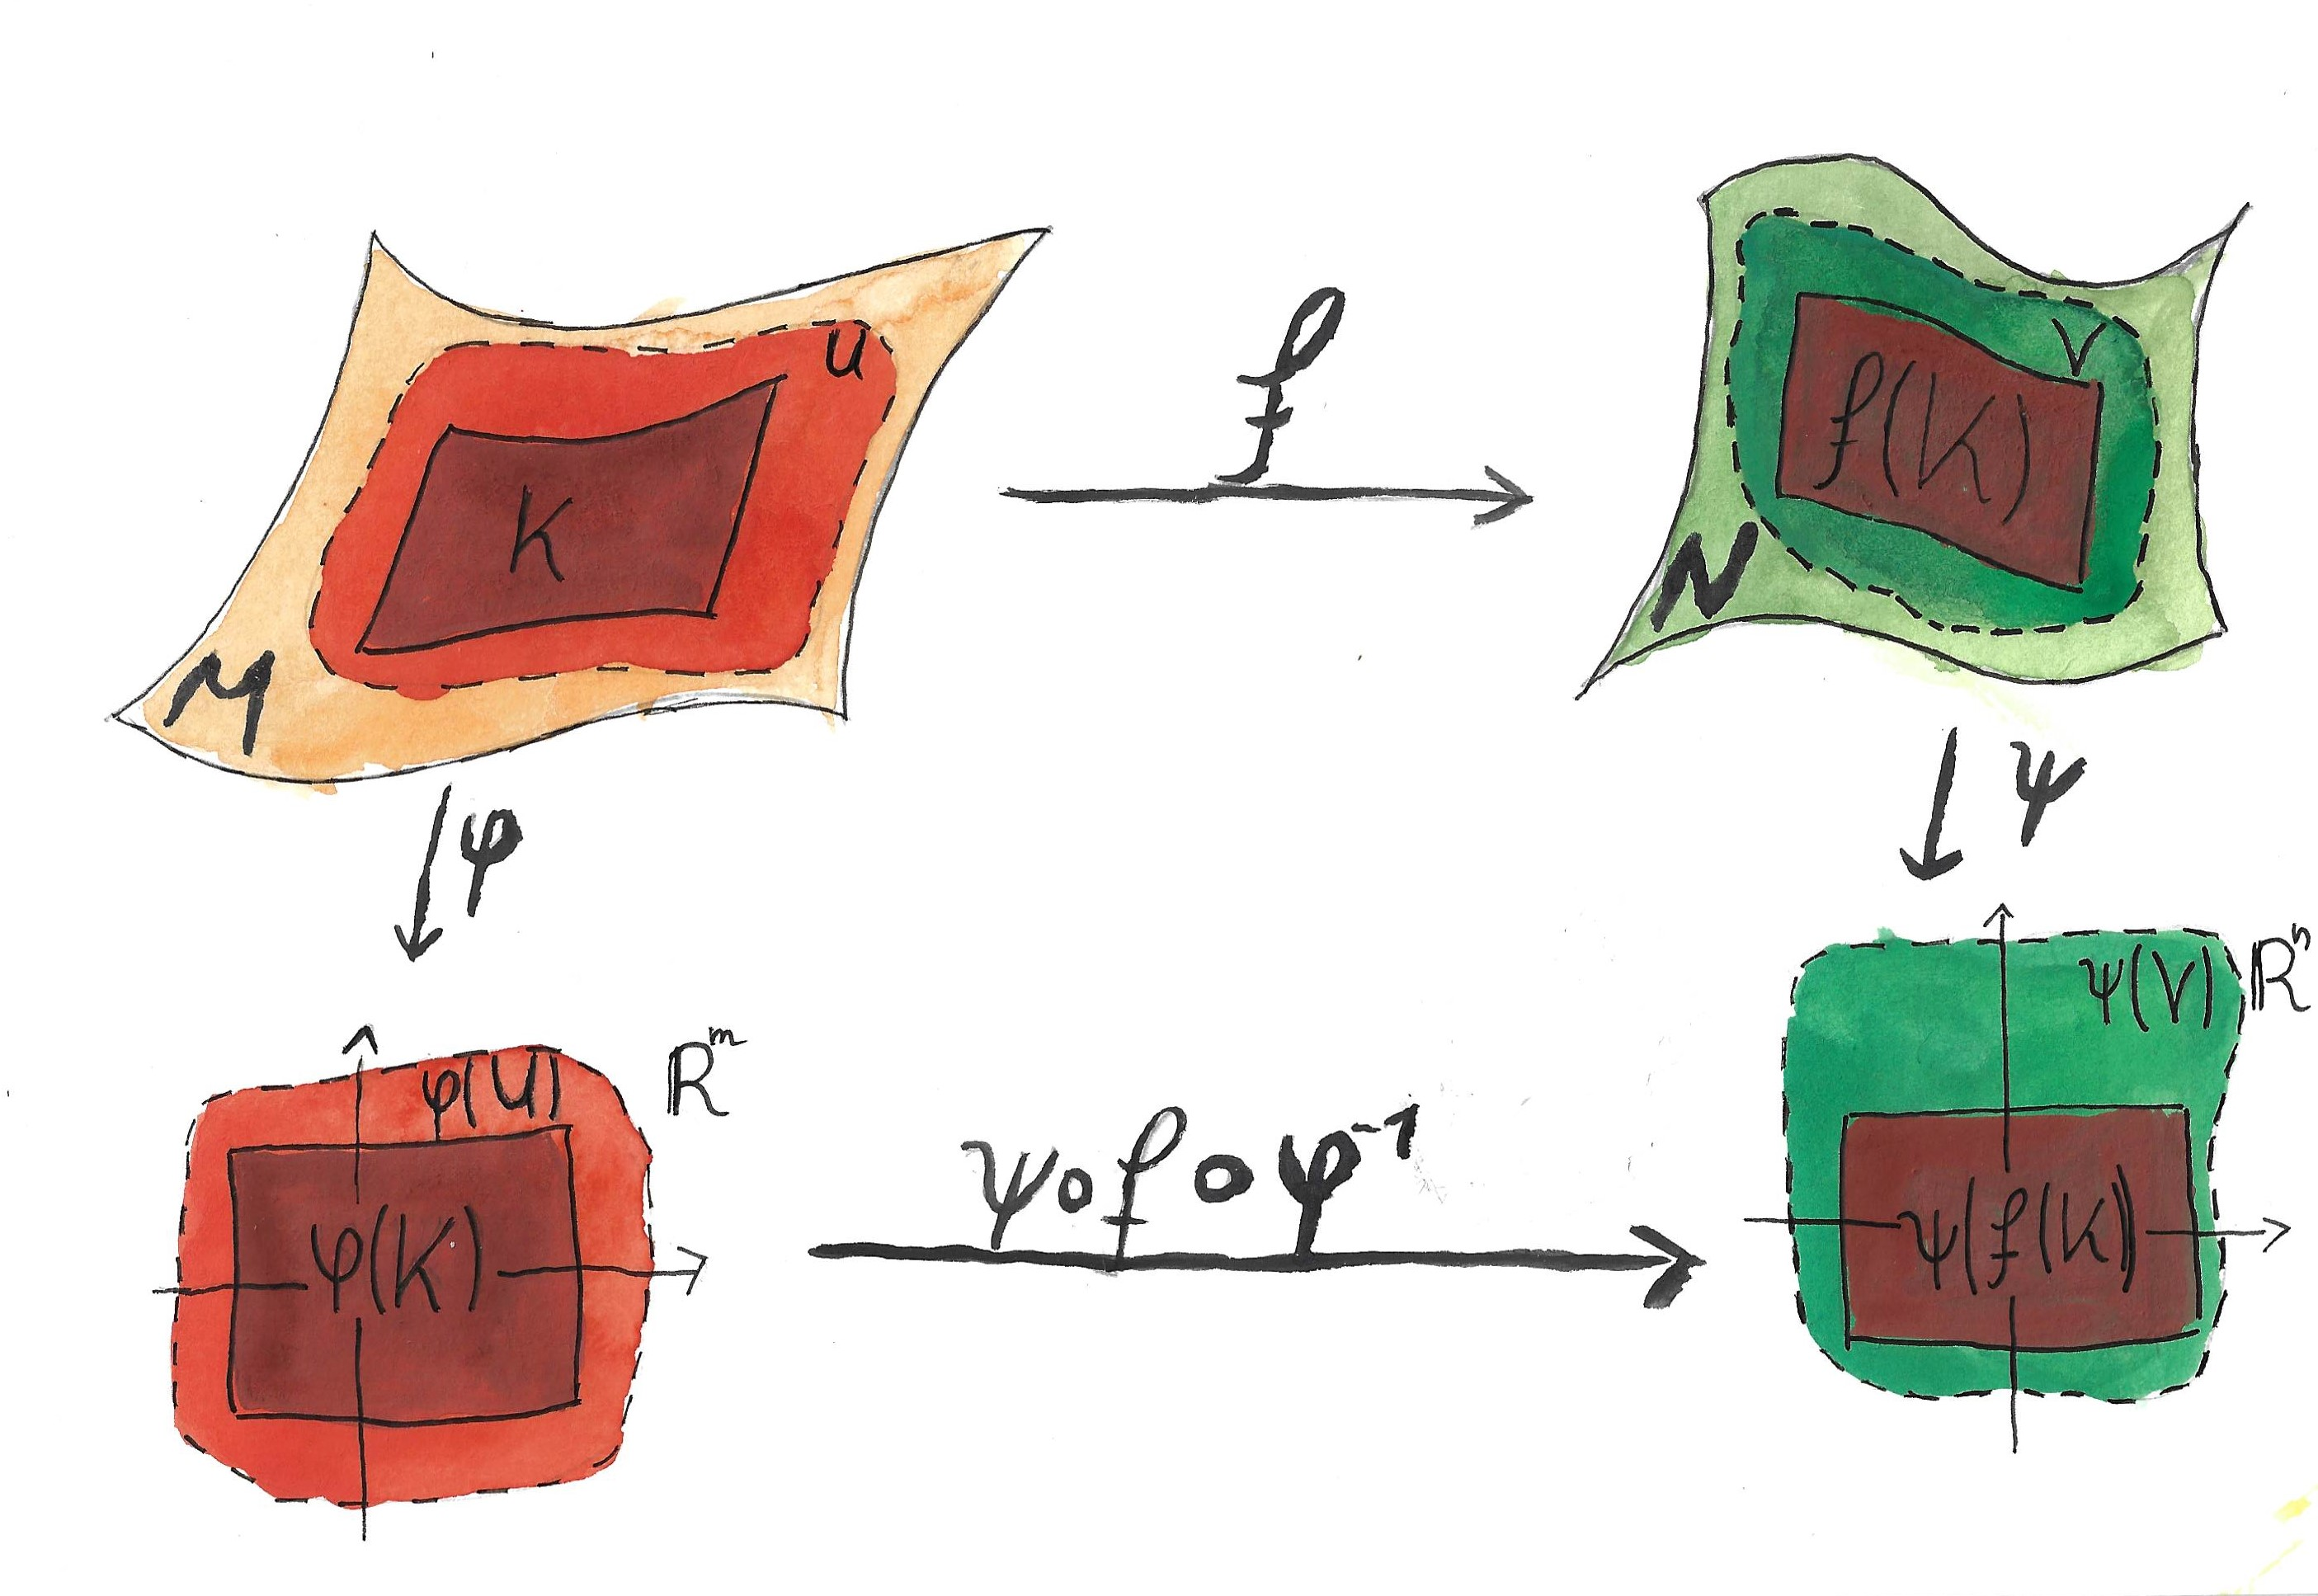
\includegraphics[width=0.7\textwidth]{Text/Pictures/lambdalemma/crTopoligie}
    \caption{The $C^r$ topology.}
    \label{fig: The C^r topology}
\end{figure} \clearpage

For $0<\epsilon\leq \infty$ the $C^r-$topology is the topology given by the subbasis:
\begin{align*}
    \mathcal{N}^r(f,(\phi,U),(\psi,V),\epsilon)  := &\{g \in C^r(M,N)| g(K) \subseteq  V   \text{ and } \\&\norm{\diff^k(\psi f  \phi^{-1})(x)-\diff ^k(\psi  g \phi^{-1})(x)}<\epsilon,~~\forall x\in \phi(K), k=0,...,r\}.
\end{align*}
\end{definition}
\begin{remark}
    The $C^1-$topology is metrizable. A proof is found in \cite{Hirsch1994} chapter 2 theorem 4.4. Now we have a metric that captures the closeness defined by the topology. 
\end{remark}
\begin{definition}[$\epsilon-$close]
Let $d_1$ be a metric that generates the $C^1-$Topology. Let $P_1,P_2,M$ be smooth manifolds and $i_{k}:P_k\to M$ for $k=1,2$ be smooth injective immersions with images 
$i_k (P_k)=W_k\subseteq M$. We call $W_1$ $\epsilon ~C^1-$ close to $W_2$ if and only if there exists a smooth map $h: P_1 \to P_2$ such that 
\begin{align*}
    d_1(i_1,i_2\circ h) <\epsilon .
\end{align*}
\end{definition}
\begin{remark}
    The idea behind the map $h$ is that two immersed manifolds respectively maps can be in proximity but have different parametrizations, such that whilst they are setwise close, pointwise they are not. With $h$ one can re-parametrize to avoid that problem.
\end{remark}
\begin{cor}\label{cor: Subspaces are also close}
If $A$ is smoothly embedded into $B$ and $B$ is $\epsilon~C^1$ close to $D$ as smoothly embedded manifolds in $M$, then $A$ is also $\epsilon~C^1$ close to $D$.
\end{cor}
\begin{proof} First let $i_b$ and $i_D$ denote the smooth injective immersions of $A$ and $D$ into $M$.
Since $B$ is $\epsilon~C^1-$close we have an $h$ such that $d(i_B,i_D\circ h)<\epsilon$. Now the $C^1$ topology cares for the pointwise closeness of the images of the maps and their derivatives. This tells us that the composition of a smooth injective immersion from the right keeps that property. In our case we can use the inclusion $i_a: A \hookrightarrow B$ to conclude that $$d(i_B\circ i_A,i_D\circ h\circ i_A)<\epsilon.$$
\end{proof}
\begin{remark}
The notion of $\epsilon~C^1-$closeness is not symmetric. By the remark above we know that a line can be epsilon close to a plane. However, the converse cannot be true since we can always find points in the plane that are not close to the chosen line. 
\end{remark}
\begin{definition}[$r-$cell]
Let $W\subseteq M$ be an immersed submanifold of $M$ with ${i:P\to i(P)=W\subseteq M}$ being the immersion. A set $B\subseteq W$ is called an \textbf{$r-$cell} if B regarded as a subset of $W$ is diffeomorphic to a closed $r-$dimensional ball. That is if $i^{-1}(B)$ is diffeomorphic to one.     
\end{definition}
\begin{theorem}[$\lambda$-Lemma]\label{thm: lambda Lemma}
    Let $W\subseteq M$ be an immersed submanifold of $M$ and let $p$ be a hyperbolic fixpoint of a diffeomorphism $\phi$ on $M$ with $\dim W(p \to)=r$ for ${0<r<m=\dim M}$. Let $N$ be an injective immersed submanifold of $M$ that is invariant under $\phi$ and has a point of transverse intersection $q$ with $W(\to p)$. Then for every $r-$cell neighborhood $B$ of $p$ in $W(p \to )$ and for every $\epsilon >0$ and for any $n\in \N_{<0}$ there is a $r-$cell $D\subseteq N$ such that $B$ is $\epsilon~C^1-$close to $D$ and there are $r-$cells $D_n\subseteq \phi^n(D)$ such that $B$ is $\epsilon~C^1-$close to $D_n$. 
\end{theorem}
\begin{remark}
We follow a proof that was given by Palais in 1969 in his thesis \cite{PalaisLambdalemma}. There are more detailes filled in by Banyaga and Hubertise in \cite{LecturesonMorseHomology}. However, there where some ambiguities in those details, when it comes to the map $h$ at the end of the proof. Here, I was able to fill those unclear parts (mainly why the projection is invertible and why that inverse is smooth) by making use of the implicit function theorem. 
\end{remark}
\begin{figure}[p!]
\centering
    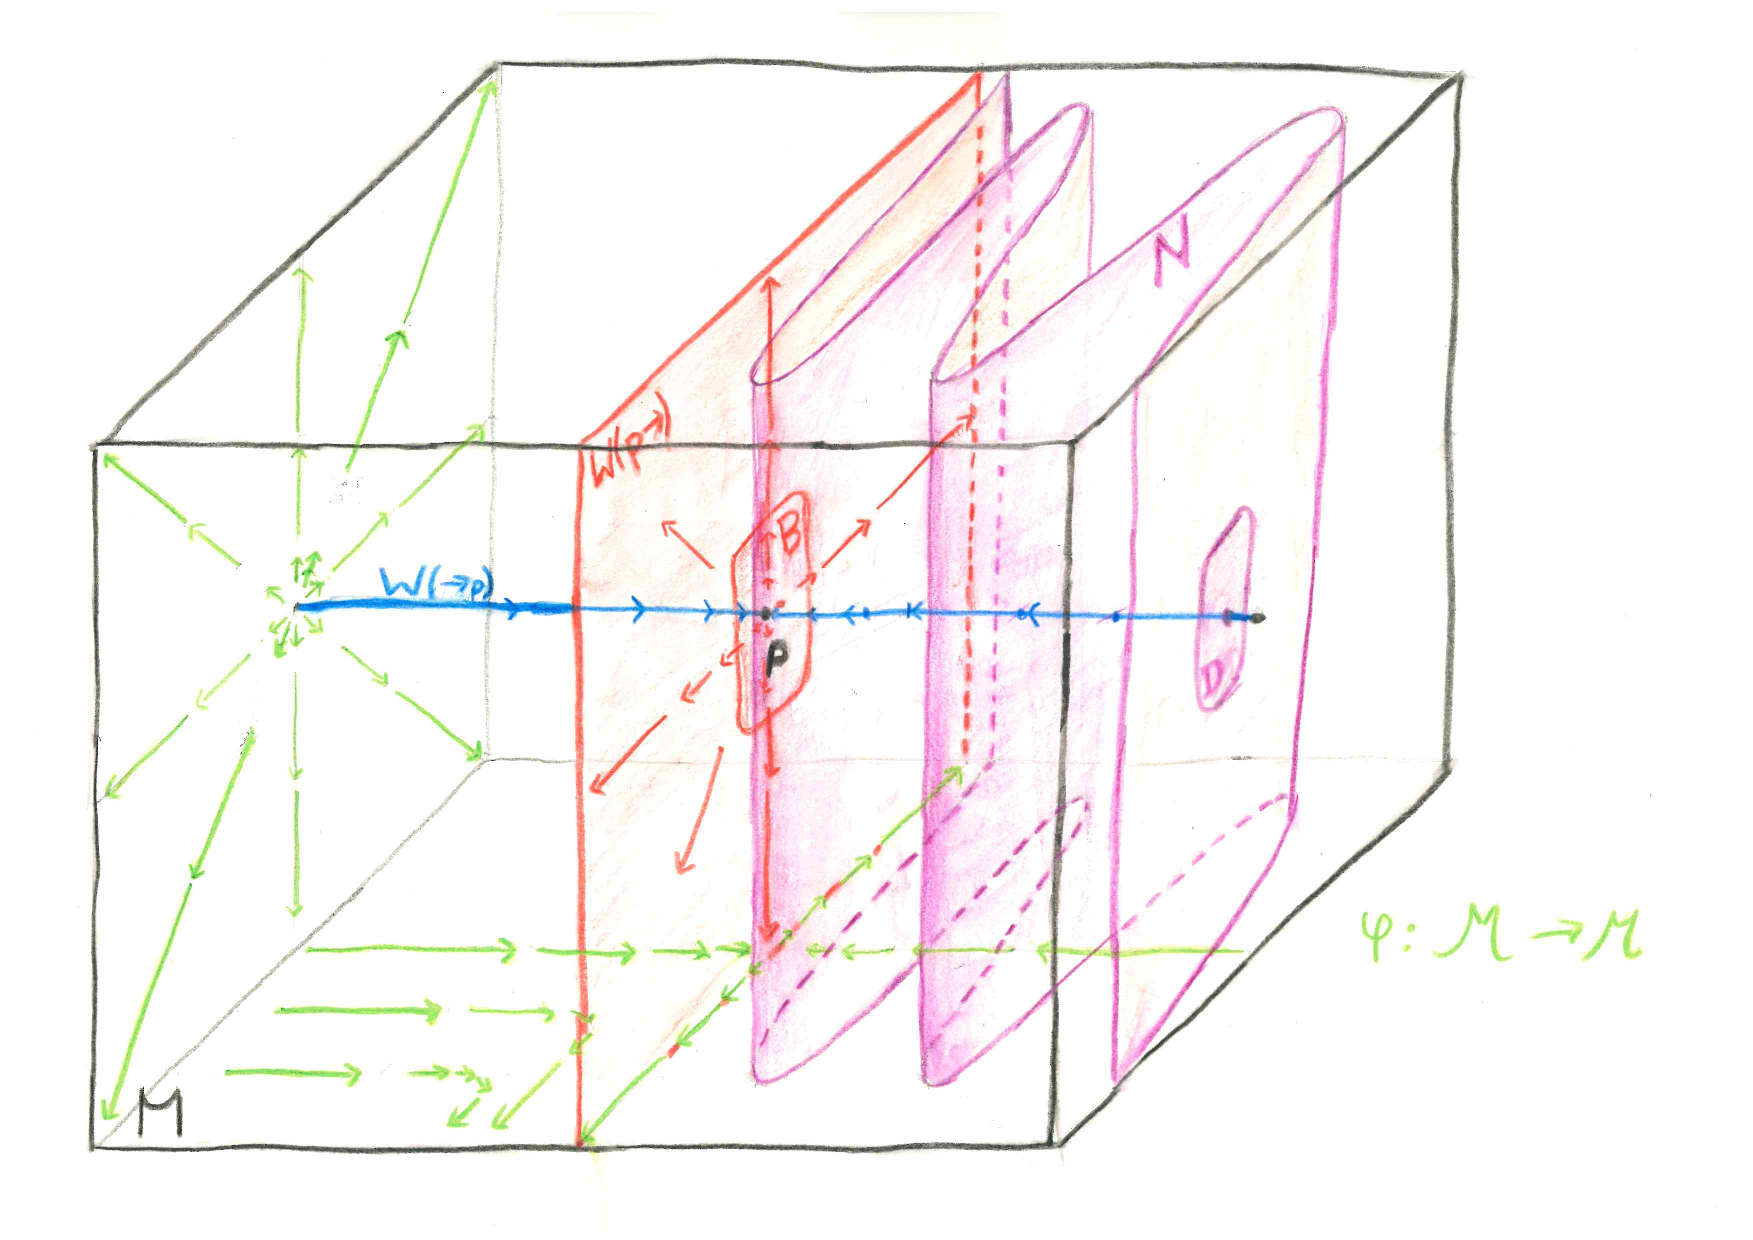
\includegraphics[width=0.956\textwidth]{Text/Pictures/lambdalemma/The lambda lemma.pdf}
    \caption{The $\lambda-$lemma.}
    \label{fig: The lambda lemma}
    In this figure the arrows that define the diffeomorphism $\phi$ are not actually drawn. The green arrows are the projected arrows onto the left side and the bottom of the cuboid. $p$ is the only fixpoint in this picture. The set N should have more layers approaching $p$ and should be a bit more deformed. Especially the layers should get wider (towards the front and back) the closer they get to $W(p \to)$ such that $N$ is invariant under $\phi$. However this picture should show the geometric nature of the statement. It is inspired by a picture in \cite{LecturesonMorseHomology} chapter 6.2 but drawn in higher dimension. 
\end{figure} \clearpage
\begin{proof}
    Let $q$ be a point of transversal intersection of $W(\to p)$ with $N$. Since $N$ and $W(\to p)$ is invariant under $\phi$ we know that $\phi^n(q)$ is also in their intersection and the intersection is again transversal since the separated tangent space $T_q W(\to p) \oplus T_qN$ in $q$ is transported to $\phi(q)$ via $\diff \phi|_q $ while the splitting is preserved. Therefore, we can assume that $q$ is contained in a chart centered at the hyperbolic fixed point $p$ respectively we can work in a neighbourhood of $0\in \R^m$ where $m=\dim M$. By the hyperbolicity we have a splitting tangent space, giving us a chart in $U$ centered at $p$ such that $U=W(\to p) \times W(p\to)\cap U$. Now since $\diff \phi|_0=\left(\begin{smallmatrix}
        A & 0\\
        0&B
    \end{smallmatrix}\right)$ we know that there is an orthogonal basis $(x_s,x_u)$ and the corresponding basis of the tangent space $(\frac{\partial}{x_s},\frac{\partial}{x_u})$ such that $\frac{\partial}{x_s}(x_u)=\frac{\partial}{x_u}(x_s)=0$. Now we make use of the fact that we are in $\R^n$ and identify the manifold and the tangent space.  With this we can Taylor expand $\phi(x_s,x_u)$ in $0$ to get $\phi(x_s,x_u)=\phi(0,0)+\diff \phi_0(x_a+x_u)+f$ where $f(0)=\diff f|_0=0$. In coordinates this reads:
    \begin{equation} \label{eq: proof of Lambda lemma phi split}
    \phi(x_s,x_u)=(Ax_s+f_s(x_s,x_u),Bx_u+f_u(x_s,x_u))
\end{equation}     Furthermore, since $f=\phi-\diff \phi|_0$ we know that: 
    \begin{align*}
        \frac{\partial f_s}{\partial x_u}|_{(0,x_u)}=\frac{\partial \phi_s}{\partial x_u}|_{(0,x_u)}=0=\frac{\partial f_u}{\partial x_s}|_{(x_s,0)}=\frac{\partial \phi_u}{\partial x_s}|_{(x_s,0)}.
    \end{align*} Similar to Corollary $\ref{cor: Tangendspace splits}$ we can define an inner product such that for the operator norm we have 
    \begin{align*}
        \norm{A}\leq \alpha <1 \quad \text{ and } \quad \norm{B^{-1}}\leq \frac{1}{\beta} <1.
    \end{align*}
    Since $1=\norm{\id}=\norm{BB^{-1}}\leq \norm{B}\cdot \norm{B^{-1}}$ we know that $\norm{B}\geq \beta$.
For a neighbourhood $U_1\subseteq U$ of the origin we define 
\begin{align*}
    k:=\max_{i,j=s,u} \Bigg\{ \sup_{\overline{U_1}}\norm{\frac{\partial f_i}{\partial x_j}} \Bigg\},
\end{align*} and choose $U_1$ small enough such that $k$ satisfies :


\begin{gather*}
0<k<1 \\
\beta_1:=\beta -k >1 \\
\alpha_1:=\alpha +k <1 \\
k<\frac{1}{4}(b_1-1)^2.
\end{gather*}
Let $B$ be a cell neighbourhood of the origin in $W(p\to )$. For some $n \in \N$ we have that $\phi^{-n}(B)\subseteq U_1$. If the $\lambda-$lemma holds for $\phi^{-n}(B)$ for all $\epsilon$ it also holds for $B$, since the metric and $\phi$ are continuous and the $r-$cell is compact. Therefore, the change of distance after applying $\phi^{-n}$ is finite and we can choose the distance from $\phi^{-n}(B)$ to $D$ small enough such that $B$ is $\epsilon~C^1$-close to $D$. Hence, without restrictions $B\subseteq U_1$ and $q\in U_1$.  Next we define the inclination of $N$ with respect to the (un-)stable manifolds as follows: 

Let $x\subseteq N \cap U_1$ and $v^0\in T_xN\subseteq T_0M=T^s_0M \oplus T^u_oM$ and let $v^0=(v_s^0,v_u^0)$ be the coordinate entries. Furthermore let $v$ be a unit vector. Now we define the \textbf{inclination} of $v^0$:
\begin{align*}
\lambda(v^0)=\frac{\norm{v^0_s}}{\norm{v^0_u}}.
\end{align*}
In other words: The smaller the inclination, the more parallel we are to $W(p\to)$. 
Furthermore define:
\begin{align*} x^n:=\phi^n(x), ~v^n:= \diff \phi_{x^{n-1}}(v^{n-1}) \text{ and } \phi(x)=(\phi_s(x),\phi_u(x))\in W(\to 0)\times W(0\to).
\end{align*}
Now we want to calculate the derivative $\diff \phi|_{q^n}$. But first inspect:
\begin{align*}
\diff \phi|_x=\begin{pmatrix}
\frac{\partial \phi_s}{\partial x_s}|_{x} & \frac{\partial \phi_s}{\partial x_u} |_{x}\\
\frac{\partial \phi_u}{\partial x_s} |_{x}& \frac{\partial \phi_u}{\partial x_u}|_{x}
\end{pmatrix}\overset{(\ref{eq: proof of Lambda lemma phi split}) }{~=~}
\begin{pmatrix}
A+ \frac{\partial f_s}{\partial x_s}|_{x}& \frac{\partial f_s}{\partial x_u}|_{x}\\
\frac{\partial f_u}{\partial x_s} |_{x} & B+ \frac{\partial f_u}{\partial x_u}|_{x}
\end{pmatrix} 
\end{align*} Since $q^n\in W(\to 0)$ and $\frac{\partial f_u}{\partial x_s}(x_s,u)$=0 this gives us:

\begin{align*}
\diff \phi|_{q^n}=\begin{pmatrix}
A+ \frac{\partial f_s}{\partial x_s}|_{q^n}&    \frac{\partial f_s}{\partial x_u}|_{q^n}\\
0                                   & B+ \frac{\partial f_u}{\partial x_u}|_{q^n}
\end{pmatrix} 
\end{align*}
Let $B_s(\delta)$ denote the ball of radius $\delta$ around the origin that lives in $W(\to p)$ and $U_2:= B_s(\delta)\times B$. Since $\frac{\partial f_s}{\partial x_u}|_{(0,x_u)}=0$ and by the smoothness of  $\phi$, for any $\epsilon >0$ there exists a $\delta$ such that 
\begin{align*}
\underbrace{\sup_{U_2}\norm{\frac{\partial f_s}{\partial x_u}}}_{:=k_1}< \min\{\epsilon, k \}.
\end{align*} This can be seen in figure \ref{fig: The definition of k_1}. 
\begin{figure}[p!]
\centering
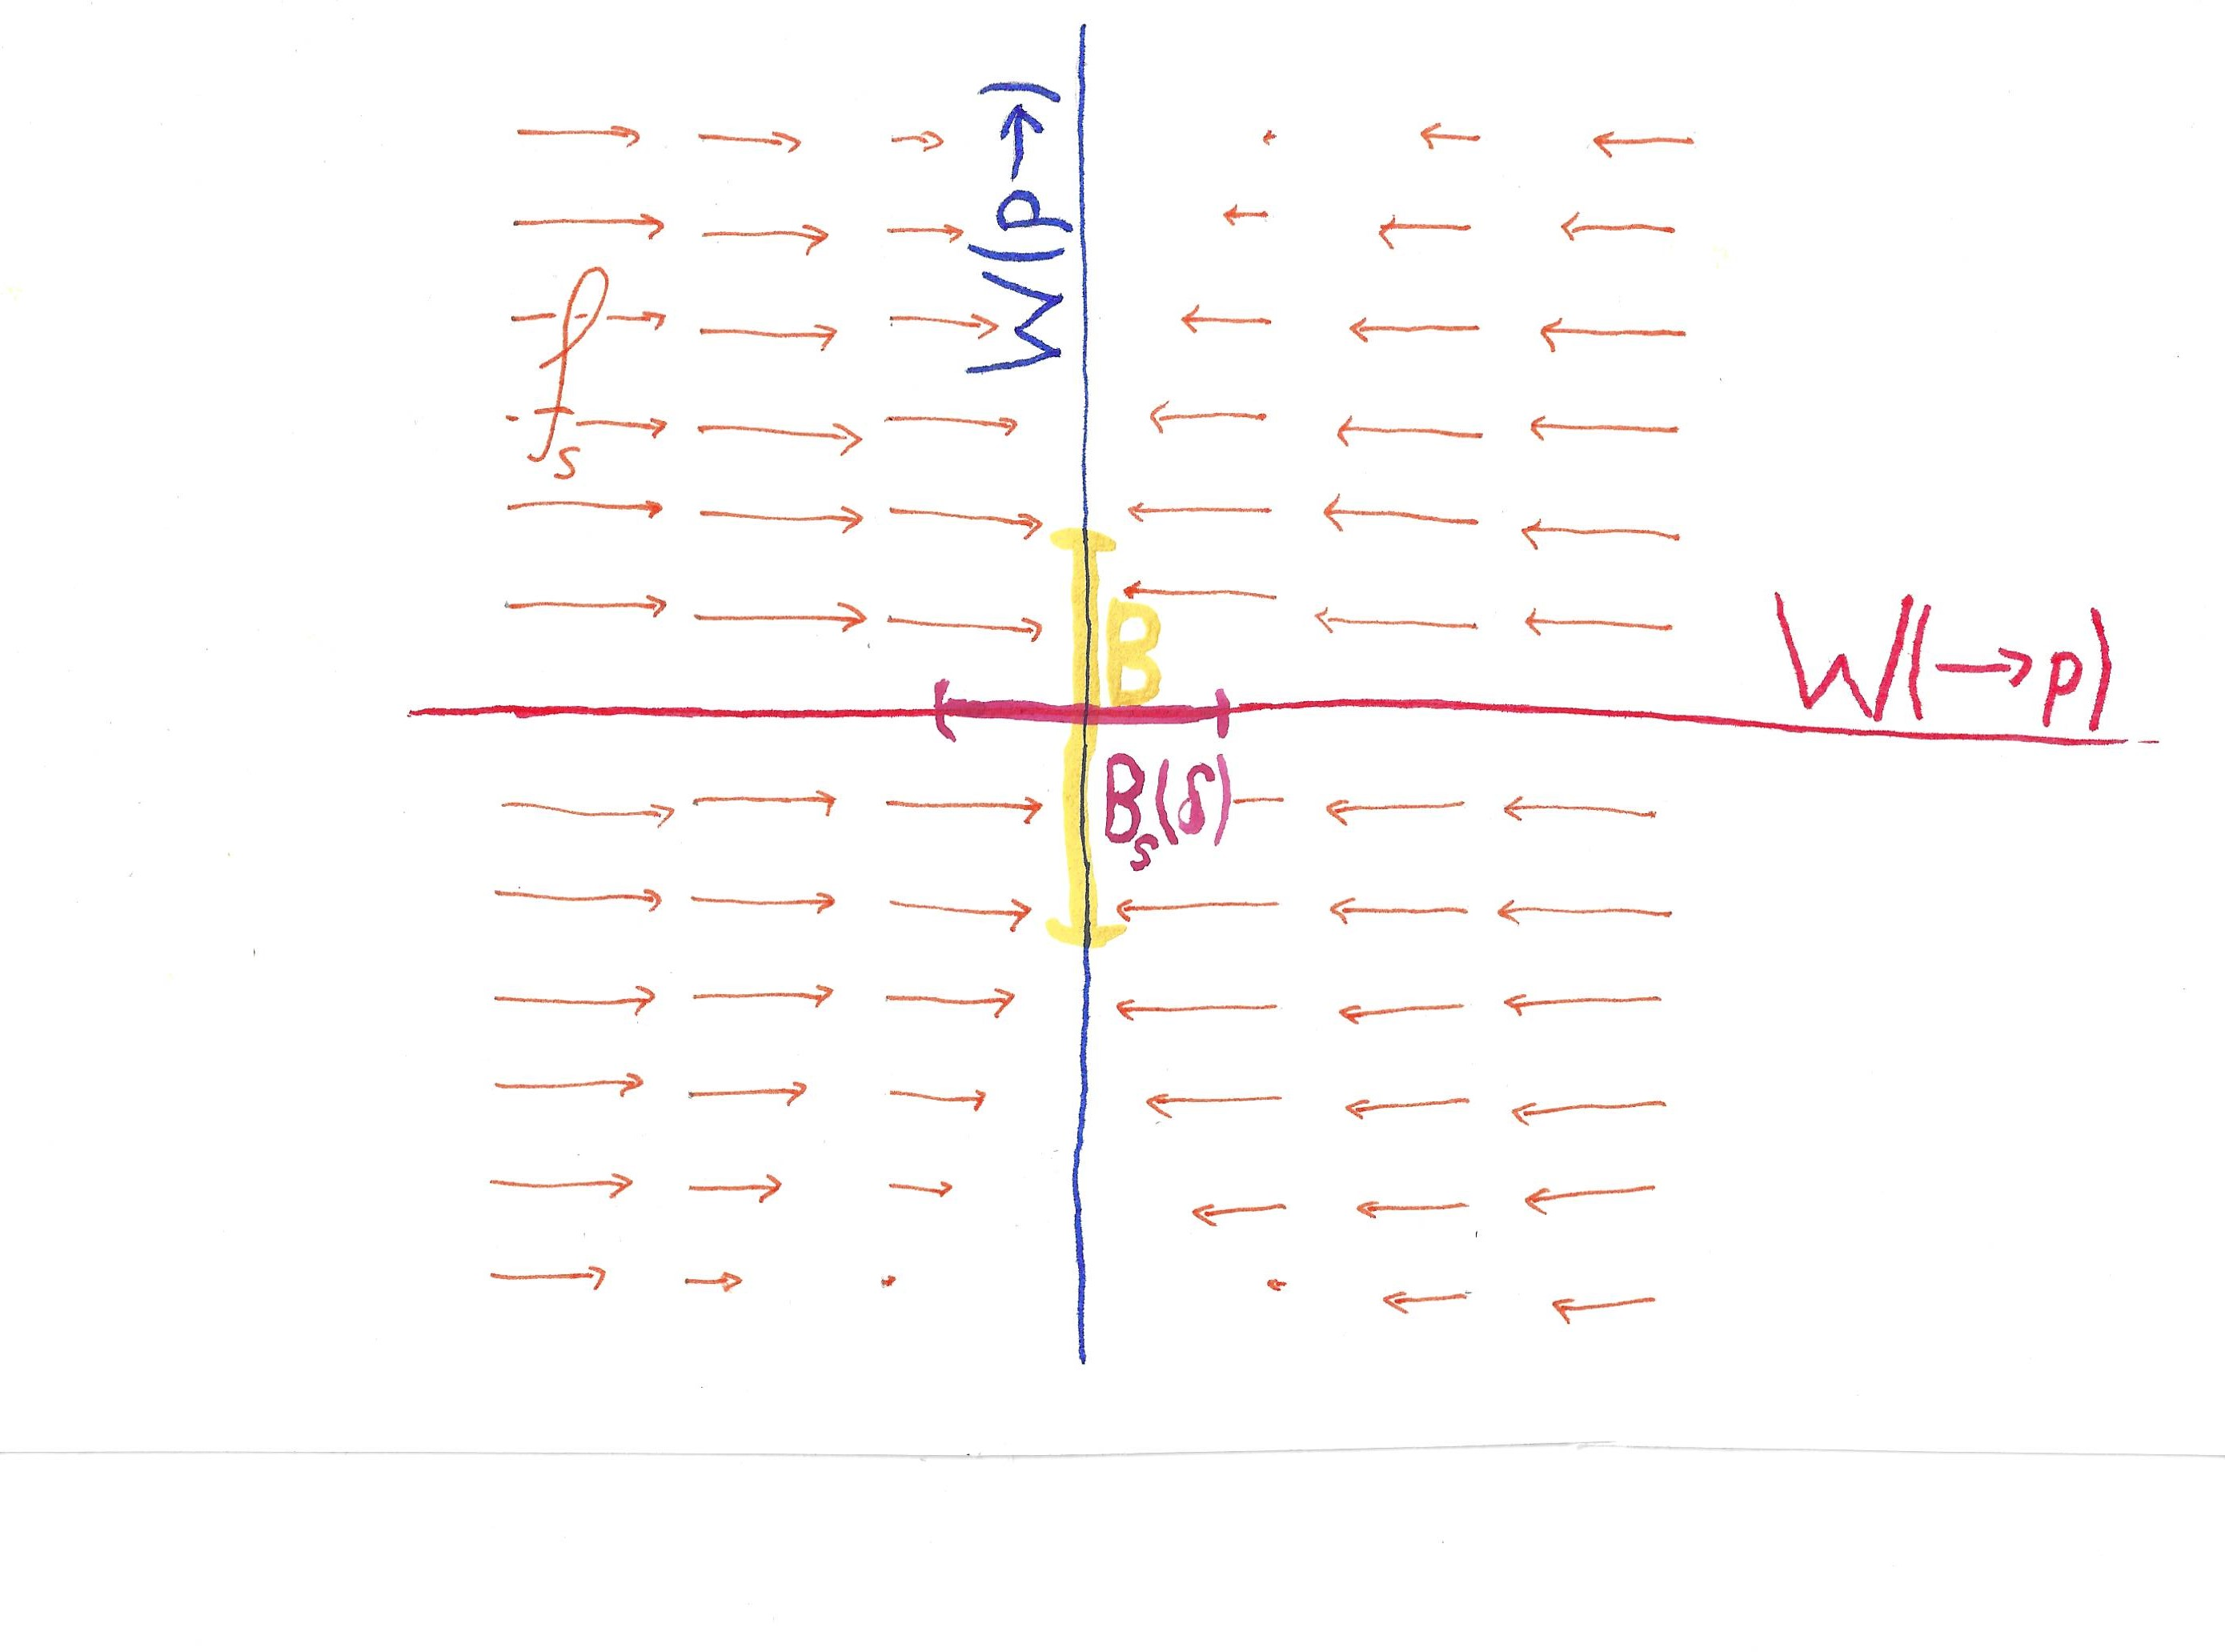
\includegraphics[width=0.6\textwidth]{Text/Pictures/lambdalemma/k1definitiin}
\caption{The definition of $k_1$.}
\label{fig: The definition of k_1}
\end{figure}\clearpage Again, we assume $q\in U_2$. Now we want to get a hold of the inclination:  Let $x\in N$ such that $x^j\in U_2 $ for all $j\leq n$ and let $v^0\in T_xN$. Denote $v^n=(v^n_s,v^n_u)\in T_0W(\to 0)\times T_0W(0 \to)$. 
\begin{align}
\lambda(v^n)&= \frac{\norm{\diff \phi_s|_{x^{n-1}}(v^{n-1})}}{\norm{\diff \phi_u|_{x^{n-1}}(v^{n-1})}} \nonumber \\
&=\frac{\norm{Av_s^{n-1} +\ \frac{\partial f_s}{\partial x_s}|_{x^{n-1}}v_s^{n-1} \ \, + \, \frac{\partial f_s}{\partial x_u}|_{x^{n-1}}(v_u^{n-1})}}{\norm{\color{blue} \frac{\partial f_u}{\partial x_s}|_{x^{n-1}}(v_s^{n-1}) \color{black}+   Bv_u^{n-1}+\frac{\partial f_u}{\partial x_u}|_{x^{n-1}}(v_u^{n-1})}} \nonumber \\
& \leq \frac{ (\alpha +k )\norm{v_s^{n-1}}+k_1 \norm{(v_u^{n-1})}}
			{ \color{blue}k \norm{(v_s^{n-1})} \color{black}  +  (\beta+k)\norm{ v_u^{n-1}}} \nonumber \\
& \leq \frac{ (\alpha +k )\norm{v_s^{n-1}}+k_1 \norm{(v_u^{n-1})}}
			{ (\beta-k)\norm{ v_u^{n-1}}  - \color{blue} k_1 \norm{(v_s^{n-1})} \color{black} } &\quad \text{since } \beta-k>1 \text{ and }k_1<k<1 \nonumber \\
& = \frac{ (\alpha +k )\lambda(v^{n-1})+k_1}
			{ \beta_1  - \color{blue} k_1 \lambda{v^{n-1}\color{black} }} &\quad \text{we divided by }\norm{v_u^{n-1}} \nonumber \\
&\leq \frac{\lambda(v^{n-1})+k_1}
			{ \beta_1  - \color{blue} k_1 \lambda(v^{n-1}) \color{black} }  \label{eq: estimate lambda(v^n)}				
\end{align} 
If $x\in W(\to 0)$ the blue part above disappears and we get:
\begin{align*}
\lambda(v^n) \leq \frac{\lambda(v^{n-1})+k_1}{\beta_1}.
\end{align*} By induction we get:
\begin{align}
\lambda(v^n)\leq \frac{\lambda(v^{n-1})+k_1}{\beta_1}=\frac{\frac{\lambda(v^{n-2})+k_1}{\beta_1}+k_1}{\beta_1}= \frac{\frac{\lambda(v^{n-2})+\frac{k_1 \beta_1}{\beta_1}}{\beta_1}+k_1}{\beta_1} =\frac{\lambda(v^{n-2})+k_1+ k_1 \beta_1}{\beta_1^2}\leq \cdots \nonumber \\
\leq \frac{\lambda(v^0)+\sum_{l=0}^{n-1}k_1 \beta_1^l}{\beta_1^n}~. \label{eq: proof lambda lemma estimate lambda(v^n) with x=q}
\end{align} By using the geometric series we see:
\begin{align*}
\lambda(v^n)\leq \frac{\lambda(v^0)}{\beta_1^n}+k_1\sum_{l=1}^n\frac{1}{\beta^n} \leq \frac{\lambda(v^0)}{\beta_1^n}+k_1(\frac{1}{1-\beta_1}-1)=
\frac{\lambda(v^0)}{\beta_1^n}+k_1(\frac{b}{\beta_1-1}-\frac{\beta_1-1}{\beta_1-1}) \\ =\frac{\lambda(v^0)}{\beta_1^n}+k_1(\frac{1}{\beta_1-1}).
\end{align*}
Since $\beta_1$ was greater then 1 we can conclude that $\lim_{n \to \infty}\frac{\lambda(v^0)}{\beta_1^n}=0$ and since $k<\frac{1}{4}(\beta_1-1)^2$ we know that $\frac{k}{\beta_1-1}<\frac{b-1}{4}$. Because of that, a $n_0$ exists such that for all $n>n_0$ :
\begin{align*}
\lambda(v^n)\leq \frac{\lambda(v^0)}{\beta_1^n}+\frac{k}{b-1}< \frac{\beta_1-1}{3}.
\end{align*}  
Lets collect what we have done so far: We take a point $x$ from a transverse intersection of $N$ and $W(\to p)$. Then, we inspect the inclination of a tangent vector $v$ in ${T_xN\subseteq T^s_0M\times T^u_0M}$ and move the tangent vector via $\diff \phi$ alongside of the stable set and realize that the inclination gets smaller, the more we move it. 






For any $v\in T_{q^n}N$ there exists a $\tilde{v} \in T_qN$ such that $v=\tilde{v}^n$, since
 $\diff \phi|_x:T_xM \to T_{\phi(x)}M$ is bijective. 
 If we take an arbitrary local section $f:M \to TM$
  that denotes the choice of $v^0\in T_xN$ we know that $\lambda \circ f$ is continuous, 
  as it is the composition of continuous functions. In other words, the inclination smoothly depends on $v^0$ and $x$. 
This tells us that for a small enough cellular neighbourhood $D_0 \subseteq N \cap U_2$ such that for any $x\in D_0$ and $v_0\in T_xN$ of length $1$ we have
\begin{equation}
\lambda(v^0)\leq \frac{1}{2} (\beta_1-1).
\end{equation}
Now we claim that if $\phi^j(v^0)\in U_2$ for all $j=0,...,n$ then $\lambda(v^n)\leq \frac{1}{2}(\beta_1-1).$ We prove this by induction: The case $n=0$ is already done. For the induction step we use the estimate (\ref{eq: estimate lambda(v^n)}), $k_1 <k<1$ and $k< \frac{1}{4}(\beta_1-1)^2$:
\begin{align*}
\lambda(v^{n+1})\leq \frac{\lambda(v^{n})+k_1}{ \beta_1  - k_1 \lambda(v^{n})}\leq \frac{ \frac{1}{2}(\beta_1-1)+\frac{1}{4}(\beta_1-1)^2}{ \beta_1  - \frac{1}{2}(\beta_1-1))} = \frac{1}{2}(\beta_1-1).
\end{align*} Using the above estimate and (\ref{eq: estimate lambda(v^n)}) again we conclude that for all $x\in D_0$ such that $\phi^j(x)\in U_2$ for all $j=0,...,n$ and for any unit vector $v^0\in T_xN$ we have:
\begin{align*}
\lambda(v^{n})& \leq \frac{\lambda(v^{n-1})+k_1}{ \beta_1  - k_1 \lambda(v^{n-1})}\\
 &\leq \frac{\lambda(v^{n-1})+k_1}{ \beta_1  - \frac{1}{2}(\beta_1-1))}\\
 &\leq \frac{\lambda(v^{n-1})+k_1}{ (\frac{1}{2}(1+\beta_1))}.
\end{align*} Notice that for $\beta_2:=\frac{1}{2}(1+\beta_1)$ we have $1<\beta_2<\beta_1$. Again like in the equation (\ref{eq: proof lambda lemma estimate lambda(v^n) with x=q}) we can use induction to conclude:
\begin{align*}
\lambda(v^n)\leq \frac{\lambda(v^0)}{\beta_2^n}+\frac{k_1}{\beta_2-1},
\end{align*} and since $k_1\leq \epsilon$ we have for any $n$ large enough, any $x\in D_0$ such that $\phi^j(x) \in U_2$ for $j=0,...,n$ and any unit vector $v^0 \in T_xN$:
\begin{align*}
\lambda(v^b)\leq \epsilon(1+\frac{1}{\beta_2-1}).
\end{align*}
Let $\pi_u:U \to W(0\to)$ be the projection. Since $\phi$ is expanding on $W(0 \to)$ we know that a $n_2\geq n_1$ exists such that $B\subseteq \pi_u(D_{n_2})$, where $D_{n_2}$ denotes the connected component of $\phi^{n_2}(D_0)\cap U$ that contains $q^{n_2}$. If $\dim N > \dim W(0 \to)$ we can choose a subset of $\dim W(0\to)$ and then the projection restricted to $D_{n_2}$:  $\pi_u|{D{n_2}}$ can be modified to be one to one. Now we need to reduce $D_{n_2}$ such that it is one to one. This turns out to be harder than expected since we need to consider problems like the set $\{(t,r\cdot \sin(\frac{1}{t}),r\cdot \cos(\frac{1}{t})|0<r\leq 1, 0<t\})$. 
However, to get rid of such problems we use the fact that we are an embedded manifold. By this we know that we are given by an implicit function where the derivatives in $W(\to p)-$direction are invertible as a matrix. By the implicit function theorem we can take any point $x$ from $D_{n_2}$ and conclude that there is a neighbourhood $U(x)\subset W(p\to)$ around $\pi_u(x)$ in $D_{n_2}$ and a smooth function $G: W(p\to)\to W(\to p)$, such that around $x$ $D_{n_2}$ looks like $(y,G(y))$ telling us that the projection onto the domain of $G$ is one to one after restricting $D_{n_2}$ to $U(x)\times \im(G)$. Now we can define $h$ to be the inverse of that projection (that is $G\times \id$) and get the closeness of $B$ to $D_{n_2}$. To see that we first check the distances and the difference after differentiating. For this we need the maps: $i_1:B\to M, x \mapsto (0,x)$, and $i_2: ~D_{n^2} \to M,~ x\mapsto x$ and $h: B \to D_{n^2},~ x \mapsto \pi_u^{-1}(x)=(h_s(x),x)=(h_s(x),h_u(x)$:

\begin{align*}
\sup_{x\in B} \norm{ \diff( i_{1} )_x-\diff (i_2 \circ h )_x} &= \sup_{x\in B} \norm{ \begin{psmallmatrix}
0 \\
 1
\end{psmallmatrix}- \begin{psmallmatrix}
\diff (h_s)_x \\
1
\end{psmallmatrix} } \\
&=\sup _{x\in B} \norm{\diff (h_s)_x } &\\
&= \sup_{x \in B} \sup_{\norm{v}\leq 1} \norm{\frac{\diff(h_s)_x}{\diff(h_u)_x}(v) \diff(h_u)_x}(v) & \text{ here:} \begin{cases} h_u \equiv  \id_{w(\to p)} \times h_u \\
h_s \equiv h_s \times \id_{W(p \to)}.
\end{cases} \\
&=\sup_{x \in B} \sup_{\norm{v}\leq 1} \frac{\norm{(\diff(h)_x)_s(v)}}{\norm{(\diff(h)_x)_u(v)}}\norm{v}\\
&= \sup_{x \in B} \sup_{\norm{v} = 1} \lambda(\diff h_x(v)) & \text{since $\diff h_x$ is linear} \\
& \leq \epsilon(1+\frac{1}{\beta_2-1}).
\end{align*} The last inequality follows from $\diff h_x(v))$ being an element in $T_xN$ and the existence of a $\tilde{v} \in D_0:\tilde{v}^n=v$. Finally since $\beta_2$ is independent of $\epsilon$ we can make this construction for any $\epsilon$. Therefore, by definition we have that for any $\mathcal{N}^r(f,(\phi,U),(\psi,V),\epsilon)$ that contains $i_2$ there is a $r-$cell $D_{n^2}$ and a $h$ such that $i_2 \circ h \in \mathcal{N}^r(f,(\phi,U),(\psi,V),\epsilon)$. This tells us that every neighbourhood of $i_1$ contains such an $h$ and therefore, in the $C^r-$generating metric $d_1$, an $r-$cell and a $h$ exists such that $d_1(i_1.i_2\circ h)<\epsilon.$ This concludes the proof of the lambda lemma.  
\end{proof} 










 
\begin{cor}\label{cor: lambda lemma first corollary} Let $M$ be a smooth manifold and suppose that $p,q$ are hyperbolic fixpoints of a diffeomorphism $\phi:M\to M$. If $W(q \to)$ and $W(\to p)$ have a point of transversal intersection, then 
\begin{align*}
W(p\to) \subseteq \overline{W(q \to )}.
\end{align*}
\end{cor}
\begin{proof}
We proof this corollary by showing that every neighbourhood of any point in $W(p\to)$ must contain elements of $W(q \to)$. The setup for this proof is the left side of figure \ref{fig: Proof of the closures of unstable sets}. Let $a\in W(p \to)$ and let $A,B \subset W(p   \to )$ be $r-$cell neighbourhoods of $a$ respectively of $p$. Notice, that there exists a $n$ such that $\phi^{-n}(A)\subseteq B$. By the $\lambda-$lemma for any $\delta$ there is a neighbourhood $D_{\delta}\subseteq W(q \to)$ such that $B$ is $\delta$ $C^1-$close to $D_{\delta}$. Since $\phi^{-n}(A)\subseteq B$ we know that $\phi^{-n}(A)$ is $\delta$ $C^1-$close to $D_{\delta}$. Thus for any $\epsilon$ we can choose a $\delta$ such that $A$ is $\epsilon~C^1-$close to $\phi^{n}(D_{\delta})$. Therefore any in $M$ open neighbourhood of $a$ contains points in $W(q\to)$.   
\end{proof}

\begin{figure}[p!]
\centering
    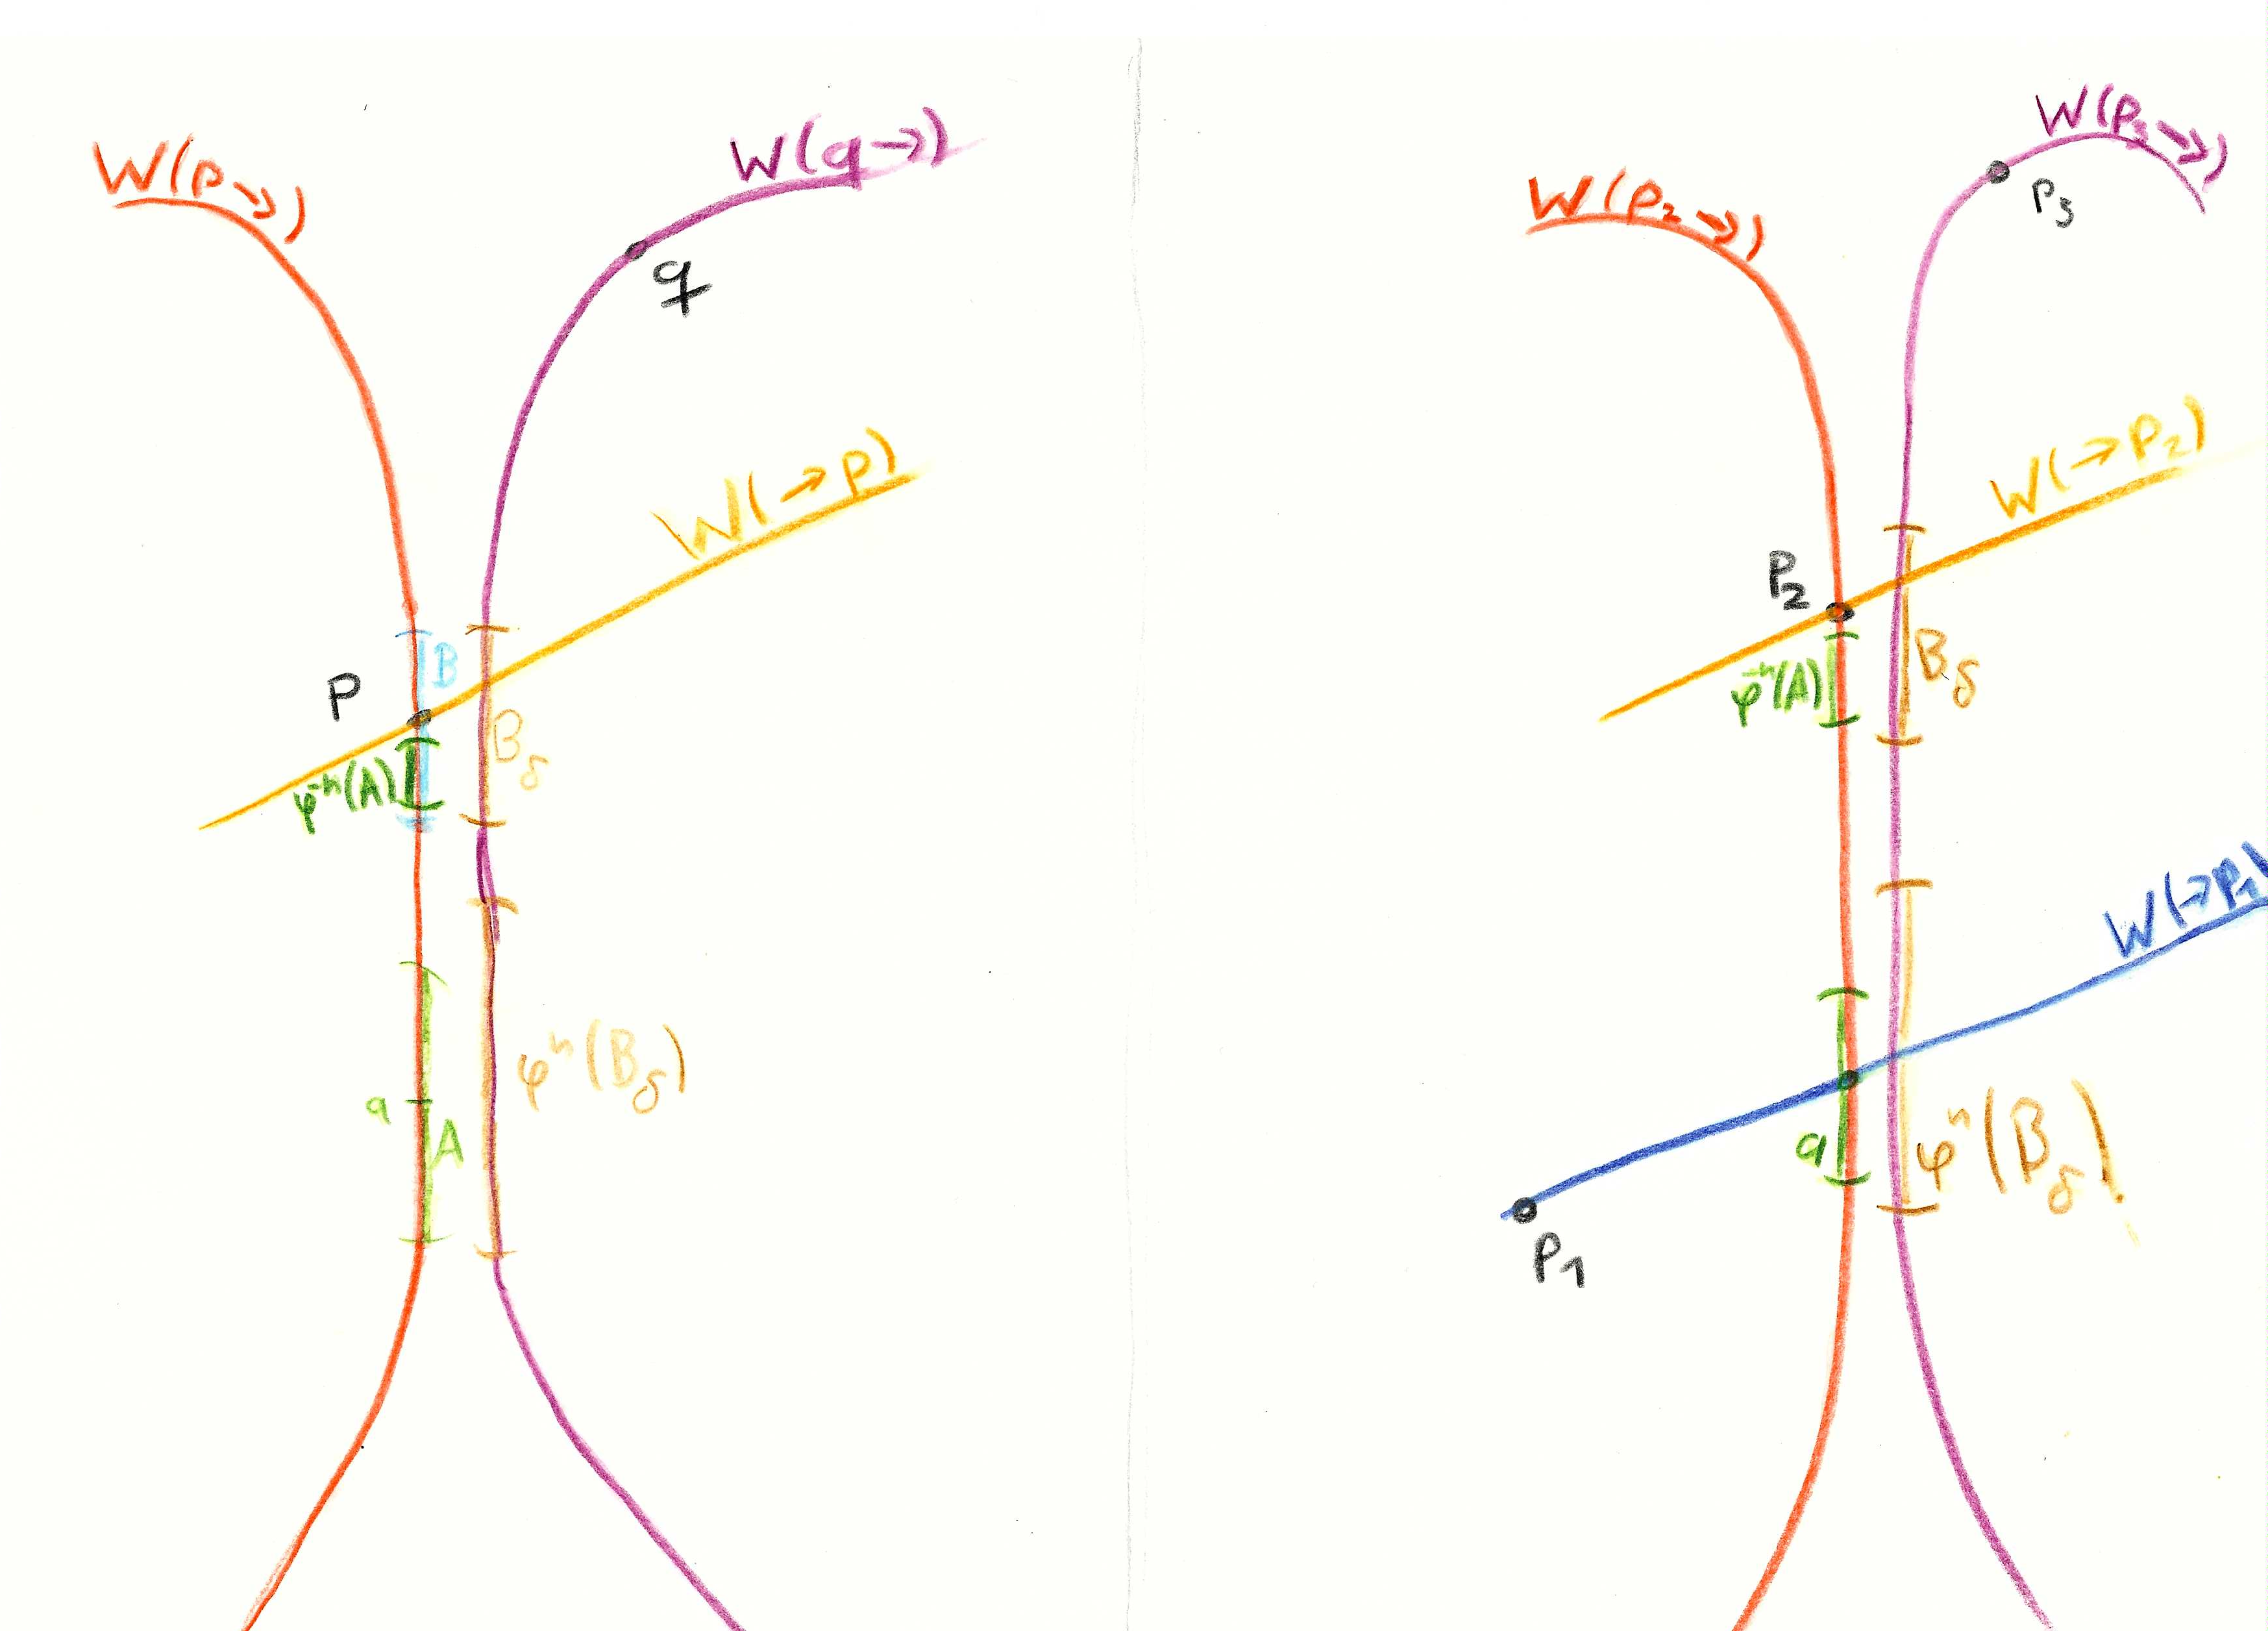
\includegraphics[width=0.9\textwidth]{Text/Pictures/lambdalemma/Cor6.16_6.17}
    \caption{Proofs of the closures of unstable sets.}
    \label{fig: Proof of the closures of unstable sets}
    The left side shows the setup for the proof of corollary \ref{cor: lambda lemma first corollary} and the right side of corollary \ref{cor: transitivity of fixpoints}.
\end{figure}\clearpage

\begin{cor}[Transitivity of gradient lines for diffeomorphisms] \label{cor: transitivity of fixpoints}
Let $M$ be a smooth manifold and suppose that $p_i$ for $i=1,2,3$ are hyperbolic fixed points of the diffeomorphism $\phi:M\to M$. Now if $W(p_3\to) $ and $ W(\to p_2)$ intersect transversally in a point and $W(p_2\to) $ and $ W(\to p_1)$ intersect transversally in a point then also $W(p_3 \to )$ and $ W(\to p_1)$. Furthermore, if $W(p_3 \to) \transcap W( \to p_2)$ and $W(p_2 \to) \transcap W(\to p_1)$ we obtain:
\begin{align*}
\overline{W(p_3 \to p_1)} \supseteq W(p_3 \to p_2) \cup W(p_2 \to p_1) \cup \{p_1,p_2,p_3\}.
\end{align*} 
\end{cor}
\begin{proof} The setup for this proof is the right side in figure \ref{fig: Proof of the closures of unstable sets}.
Let $a$ be in the transverse intersection of $W(p_2 \to )$ and $W(\to p_1 )$. Let $A\subseteq W(p_w \to)$ be an $r-$cell neighbourhood of $a$ and $B\subseteq W(p_2\to)$ one of $p_2$ where $\dim W(p_2 \to)=r$. Then by the same argument as in the proof of corollary \ref{cor: lambda lemma first corollary} we have that for arbitrary $\epsilon>0$ there exists an $D_\delta \subseteq W(p_3 \to)$  such that $A$ is $\epsilon~C^1-$close to $\phi^n(D_{\delta})$. Since $A$ has a point of transverse intersection with $W(\to p_1)$ there is an $\epsilon>0$ such that $A$ and $\phi^n(D_{\delta})$ intersect transversally. That is because the property of having a transverse intersection is locally stable.

Now assume that $W(p_3 \to) \transcap W(\to p_2)$ and $W(p_2 \to) \transcap W(\to p_1 )$. As above we can conclude that for any $a\in W(p_2 \to) \cap W(\to p_1 )=W(p_2 \to p_1)$ we can choose an $r-$cell $A\subseteq W( p_2\to)$ that is arbitrary close to a cell in $W(p_3 \to)$ that also contains a transverse intersection with $W(\to p_1)$. In other words: For any element in $W(p_2 \to p_1)$ there is an arbitrary close element in $W(p_3 \to p_1)$, telling us that:
\begin{align*}
\overline{W(p_3 \to p_1)} \supseteq W(p_2 \to p_1).
\end{align*} Now to get $\overline{W(p_3 \to p_1)} \supseteq W(p_3 \to p_2)$, we will look at $\phi^{-1}$. Notice that $W(p_3 \to p_1)=W_{\phi^{-1}}(p_1 \to p_3)$, where the latter denotes the same intersection of the (un-)stable manifoldes with respect to $\phi^{-1}$ instead of $\phi$. With that idea and the same argument as above we find:
\begin{align*}
\overline{W(p_3 \to p_1)}=\overline{W_{\phi^{-1}}(p_1 \to p_3)}\supseteq W_{\phi^{-1}}(p_2 \to p_3)=W(p_3 \to p_2).
\end{align*} Finally, since a closed space contains all limits we know that $p_3,p_2$ and $p_1$ is also contained. This concludes the proof. 
\end{proof}

For now $M$ will be a smooth compact Riemannian manifold and $f:M \to \R$ a Morse-Smale function. In this setting we have the following corollaries:
\begin{cor}[Transitivity of gradient lines for critical points] \label{cor: lambda lemma transitivity of critical points}
Let $p,q,r$ be critical points of $f$ such that $W(r \to q)\neq \emptyset$ and $W(q\to p) \neq \emptyset$. Then we have that $W(r \to p)\neq \emptyset$, and 
\begin{align*}
\overline{W(r \to p)}\supseteq W(r \to q)\cup W(q \to p) \cup \{p,q,r\}.
\end{align*} 
\end{cor}
\begin{definition} Let $p,q,r$ be critical points of a Morse-Smale function on a smooth compact Riemannian manifold. We say that $q$ \textbf{succeeds} $r$, if $W(r \to q)\neq \emptyset$ and write $p\succeq q$. With this definition we have that $(\Crit_f(M),\succeq)$ is a partially ordered set called the \textbf{face diagram}. The face diagramm of the torus can be seen in figure \ref{fig: Definition of the filtration}.
\end{definition}
\begin{cor}
The pair $(\Crit_f(M), \succeq)$ is a partial ordered set.
\end{cor}
\begin{proof}
We need to check three properties:
\begin{enumerate}
\item \textit{Reflexivity} is clear, since $W(p \to p)=\{p\}$.
\item \textit{Antisymmetry} follows from the fact that Morse functions decrease along gradient lines. The latter can be shown locally in one chart and extended via transitivity of the order of $\R$. Locally this is clear, as the function $f$ is smooth and $-\grad$ points in the direction of the biggest decrease. 
\item \textit{Transitivity} was proven above.
\end{enumerate}
\end{proof}
\begin{cor}\label{cor: lambda lemma corollary a} For any critical point $q$ of $f$ we have that
\begin{align*}
\overline{W(q\to)}\supseteq \bigcap_{\{p \in \Crit_f(M) | ~p \succeq q\}} W(p \to).
\end{align*} If $p \succeq q$ then we can extend it to
\begin{align*}
\overline{W(q \to p)}\supseteq \bigcap_{\{\tilde{q},\tilde{p} \in \Crit_f(M) |~ q \succeq \tilde{q} \succeq \tilde{p} \succeq p \} }W(\tilde{q} \to \tilde{p})
\end{align*}
\end{cor}
\begin{proof}
This is a reformulation of corollary \ref{cor: transitivity of fixpoints}.
\end{proof}
Next we want to get equalities in the corollary above. For this two more lemmas are required:
\begin{lemma} \label{lemm: lambda lemma p is in W(q to )}
If $\overline{W(q\to)}\cap W(p\to)\neq \emptyset$, then $p$ is contained in $\overline{W(q \to )}$.
\end{lemma}
\begin{proof}
For $x\in \overline{W(q \to)}$ we have that $\phi_t(x)$ for any real $t$ is still contained in $\overline{W(q \to)}$ and since it is closed we can also take limits. So if we take $x\in \overline{W(q\to)}\cap W(p \to)$ we can conclude that \begin{align*}
p=\lim_{t\to - \infty} x \quad \in ~\overline{W(q \to)}.
\end{align*}
\end{proof}
\begin{lemma}\label{lemm: lambda lemma p is in W(q to )2}
If $p\neq q$ are critical points such that $p\in \overline{W(q \to)}$, then $\overline{W(q\to)}$ intersects $W(\to p)\setminus \{p\}$.
\end{lemma}
\begin{proof}
Since $f$ is a Morse function we can choose a small neighbourhood of $p$ in $M$ such that $p$ is the only contained critical point in $\overline{U}$. Now if $W(q \to p) \neq \emptyset$ we are done by corollary \ref{cor: lambda lemma flow lines have decreasing index}. But if the intersection is empty we can search for an intersection in the following elegant way: 
Choose a sequence $(x_j)_{j\in \N}$ such that all $x_j\in (W(q\to )\cap U) \setminus \{p\}$ are on a distinct flow line and converge to $p$. For each $x_j$ we define $k_j\in  \N$ to be the smallest natural number such that $\phi^{-k_j}(x_j)\notin U$. Since $k_j$ is minimal we also have that for any $k>0$:
\begin{align} \label{eq: lambda lemma proof of a lemma }
\phi^k(\phi^{-k_j}(x_j))\in U. 
\end{align}
 Now we have that $\lim_{j\to \infty}k_j=\infty$. Since $M$ is compact and $\overline{W(\to q)}$ is closed we know that it is also compact and therefore the series $(\phi^{-k_j}(x_j))_j$ has a limit point $x\in \overline{W(\to q)}$. After restricting to a subsequence we can assume that $\lim_{j\to \infty} \phi^{-k_j}(x_j)=x$. We now want to show that $x\in W(\to p)$. Notice that $\lim_{j \to \infty}\phi^k(\phi^{k_j}(x_j))=\phi^k(x)$ and by (\ref{eq: lambda lemma proof of a lemma }) we have that $\phi^k(x)\in \overline{U}$ for all $k$. Therefore, $x$ needs to be in the stable set of $p$, as otherwise it would converge to some other critical point in $\overline{U}$, which does not exist. Furthermore, since $x$ is not in $U$ it cannot be $p$ and this concludes the search for an intersection different from $p$.  
\end{proof}
\begin{cor} \label{cor: lambda lemma corollary b}
Let $p,q$ be critical points of $f$. If $\overline{W(q \to)}\cap W(p \to) \neq \emptyset$, then $q \succeq p$.
\end{cor}
\begin{proof}
We prove this by constructing a chain in the partially ordered $(\Crit(f),\succeq)$ that starts in $p=p_1$ and ends in $q$. For this we construct the following algorithm: 
\begin{enumerate}
\item Since $\overline{W(q \to)}\cap W(p_1 \to) \neq \emptyset$ we conclude by lemma \ref{lemm: lambda lemma p is in W(q to )} that $p_1 \in \overline{W(q \to)}$.
\item  With lemma \ref{lemm: lambda lemma p is in W(q to )2} we conclude that there is a $x\in \overline{W(q \to})\cap(W(\to p_1)\setminus \{p_1 \})$. By lemma \ref{lem: start and finish in critical points} we know that $x\in W(p_2\to)$ for some critical point $p_2 \neq p_1$. Notice that this is true if and only if $p_1 \neq q$. Therefore, $\overline{W(q \to)}\cap W(p_2 \to ) \neq \emptyset$ and we can repeat the first step with $p_2$.
\end{enumerate}
The recipe above leads to the chain $\cdots p_k \succeq p_{k-1} \succeq \cdots p_1=p$. Since there are only finitely many critical points, this terminates eventually which means that at one point $p_k=q$ and the transitivity tell us, that $q\succeq p$.
\end{proof}
\begin{cor}\label{cor: lambda lemma closer of (un-)stabnle sets}
For any critical point $q$ of $f$ we have:
\begin{align*}
\overline{W(q \to)}=\bigcup_{q \succeq p} W(p \to), 
\end{align*}and 
\begin{align*}
\overline{W(\to q )}=\bigcup_{r \succeq q} W(\to r). 
\end{align*}
\end{cor}
\begin{proof}
For the first equation, \glqq $\supseteq$ \grqq~ is just corollary \ref{cor: lambda lemma corollary a}. To show the other inclusion we take an element $x\in \overline{W(q \to)}$. This $x$ is contained in some $W(p \to)$ and therefore we have that $\overline{W(q \to)} \cap W(p \to)\neq \emptyset$. With corollary \ref{cor: lambda lemma corollary b} we can conclude that $q\succeq p$ and therefore $W(p \to)$ is contained in the right union telling us that $x$ is contained in the union. \\
For the second equation notice how it is the first equation if one considers $-f$ instead of $f$. 
\end{proof}
\begin{cor} If $p$ and $q$ are critical points and $q \succeq p$, then 
\begin{align*}
\overline{W(p \to q)}=\overline{W(q\to)}\cap \overline{W(\to p)}=\bigcup_{q \succeq \tilde{q} \succeq \tilde{p}\succeq p } W(\tilde{q} \to \tilde{p}).
\end{align*} The union here is to be interpreted like the union in corollary \ref{cor: lambda lemma corollary a}.
\end{cor}
\begin{proof}
It is obvious, that ${\overline{W(q\to p)}\subseteq \overline{W(q\to)}\cap \overline{W(\to p)}}$, since $$W(q \to p)=W(q\to)\cap W(\to p).$$ For the other containment take $x\in \overline{W(q\to)}\cap \overline{W(\to p)}$. By the corollary \ref{cor: lambda lemma closer of (un-)stabnle sets} we can take a $q_2 \in \Crit_f(M)$ such that $q \succeq q_2$ and $x\in W(q_2 \to)$ and a $p_2\in \Crit_f(M)$ such that $p_2 \succeq p$ and $x\in W(\to p_2)$. Therefore, $x\in W(q_2\to p_2)$ letting us deduce that $q_2\succeq p_2$.
By corollary  \ref{cor: lambda lemma transitivity of critical points} we can conclude that:

\begin{align*}
\overline{W(q\to p_2)}\supseteq W(q\to q_2)\cap W(q_2 \to p_2),  
\end{align*} and therefore contains $x$. Furthermore, since by the same corollary $$\overline{W(q\to p)}\supseteq W(q \to p_2).$$ This containment still holds after closing the latter we deduce that $x\in \overline{W(q\to p)}. $
This concludes the first equality of the statement. The second one is just a calculation:
\begin{align*}
\overline{W(q\to)}\cap \overline{W(\to p)} &= \bigcup_{q \succeq \tilde{q}} W(\tilde{q} \to) \cup \bigcup_{\tilde{p} \succeq p} W(\to \tilde{p})\\
&=  \bigcup_{q \succeq \tilde{q}, \tilde{p} \succeq p} W(\tilde{q} \to) \cup W(\to \tilde{p})\\
&= \bigcup_{q \succeq \tilde{q} \succeq \tilde{p} \succeq p} W(\tilde{q} \to  \tilde{p})
\end{align*}
\end{proof}
\vspace*{30mm}
\begin{minipage}{\textwidth}
\begin{centering}
\rule{0.3\textwidth}{0.4pt} \\
\textit{ The next chapter tries to connect\\
two critical points with index one apart\\
and one more generic condition needs to be choosen smart\\
so that the theory is simple, that we get. \\
We force the (un-) stable set to intersect transversal\\
and then deduce that universal:\\
"If there is a flow invariant set intersecting the stable set transversally,\\
it is pointwise close to the unstable set and their inclinations almost agree".\\
This lets us conclude a list of corollary\\
that tell us how the closure of the (un-)stable sets come to be.\\
~\\}
\end{centering}
\end{minipage}

